% =====================================================================
%  FinNLP 2026 poster -- A0 portrait (841 x 1189 mm)
%  Build:  cd poster && pdflatex -interaction=nonstopmode poster.tex
%  Palette and icon language are inherited from blog/pipeline.tex so the
%  poster and the paper figure read as one piece.
% =====================================================================
\documentclass{article}

\usepackage[paperwidth=841mm,paperheight=1189mm,margin=38mm,footskip=0pt]{geometry}
\usepackage[T1]{fontenc}
\usepackage[utf8]{inputenc}
\usepackage{helvet}
\renewcommand{\familydefault}{\sfdefault}
\usepackage{inconsolata}
\usepackage{graphicx}
\usepackage{booktabs}
\usepackage{microtype}
\usepackage{tikz}
\usetikzlibrary{positioning, calc}

\definecolor{ink}{HTML}{1A1F26}
\definecolor{muted}{HTML}{6B7480}
\definecolor{teal}{HTML}{0F6E63}
\definecolor{tealsoft}{HTML}{E2F0ED}
\definecolor{rulec}{HTML}{D5DAE1}
\definecolor{warm}{HTML}{9A5B12}

\color{ink}
\pagestyle{empty}
\setlength{\parindent}{0pt}
\setlength{\parskip}{6mm}
\renewcommand{\arraystretch}{1.35}

% ---------- type scale for A0 ----------
\newcommand{\TitleF}{\fontsize{86}{96}\selectfont\bfseries}
\newcommand{\SubtitleF}{\fontsize{46}{56}\selectfont}
\newcommand{\BylineF}{\fontsize{30}{40}\selectfont}
\newcommand{\HeadF}{\fontsize{38}{46}\selectfont\bfseries}
\newcommand{\BodyF}{\fontsize{26}{36}\selectfont}
\newcommand{\SmallF}{\fontsize{22}{30}\selectfont}
\newcommand{\TabF}{\fontsize{24}{32}\selectfont}

% ---------- building blocks ----------
\newcounter{sec}
\newcommand{\heading}[1]{%
  \vspace{1mm}%
  {\color{teal}\rule{\linewidth}{2.4pt}}\par\vspace{2mm}%
  \stepcounter{sec}%
  {\HeadF\textcolor{teal}{\thesec.}~#1\par}\vspace{-2mm}}

\newcommand{\panel}[2][tealsoft]{%
  \begin{tikzpicture}
    \node[fill=#1, rounded corners=6pt, inner sep=7mm,
          text width=\dimexpr\linewidth-16mm\relax, align=left] {#2};
  \end{tikzpicture}}

\newcommand{\takeaway}[1]{{\BodyF\itshape\textcolor{teal}{#1}\par}}

% Horizontal bar with a value label at its end, for the ablation chart.
% #1 y-offset (mm)  #2 value (0-100)  #3 row label  #4 bar color
\newcommand{\abbar}[4]{%
  \node[anchor=south west, font=\SmallF, text=ink] at (0,#1+5.5) {#3};
  \draw[fill=#4, draw=none] (0,#1) rectangle (#2,#1+5);
  \node[anchor=west, font=\SmallF\bfseries, text=ink] at (#2+2,#1+2.5) {#2\%};
}
% Horizontal bar plus a 95% CI whisker, for the model-comparison chart.
% #1 y-offset  #2 accuracy  #3 CI low  #4 CI high  #5 row label  #6 bar color
\newcommand{\modbar}[6]{%
  \node[anchor=south west, font=\SmallF, text=ink] at (0,#1+5.5) {#5};
  \draw[fill=#6, draw=none] (0,#1) rectangle (#2,#1+5);
  \draw[ink, line width=0.5pt] (#3,#1+2.5) -- (#4,#1+2.5);
  \draw[ink, line width=0.5pt] (#3,#1+1.2) -- (#3,#1+3.8);
  \draw[ink, line width=0.5pt] (#4,#1+1.2) -- (#4,#1+3.8);
  \node[anchor=west, font=\SmallF\bfseries, text=ink] at (#4+2,#1+2.5) {#2\%};
}
\newcommand{\baraxis}{%
  \draw[rulec] (0,-4) -- (100,-4);
  \node[anchor=north, font=\SmallF, text=muted] at (0,-4) {0};
  \node[anchor=north, font=\SmallF, text=muted] at (50,-4) {50};
  \node[anchor=north, font=\SmallF, text=muted] at (100,-4) {100\%};
}
% Small integer-count bar (max 4), for the error-type breakdown.
% #1 y-offset  #2 count  #3 row label
\newcommand{\errbar}[3]{%
  \node[anchor=south west, font=\SmallF, text=ink] at (0,#1+5.5) {#3};
  \draw[fill=teal!70, draw=none] (0,#1) rectangle (#2,#1+5);
  \node[anchor=west, font=\SmallF\bfseries, text=ink] at (#2+0.1,#1+2.5) {#2};
}

\newlength{\colw}
\setlength{\colw}{0.315\textwidth}
\newlength{\colgap}
\setlength{\colgap}{0.0275\textwidth}
% Width spanning two adjacent columns (same for any pair -- all columns and
% gaps are equal width). Used once for the map (columns 1+2, at the bottom)
% and once for the walkthrough figure (columns 2+3, at the top).
\newlength{\twocolw}
\setlength{\twocolw}{\dimexpr 2\colw+\colgap\relax}

\newlength{\mapdispw}
\setlength{\mapdispw}{\dimexpr \twocolw*90/100\relax}
\newlength{\mapht}
\setlength{\mapht}{\dimexpr \mapdispw*19584/47520\relax}

\newlength{\wtdispw}
\setlength{\wtdispw}{\dimexpr \twocolw*92/100\relax}
\newlength{\wtht}
\setlength{\wtht}{\dimexpr \wtdispw*87008/484202\relax}
% Left margin that centers the (narrower-than-twocolw) walkthrough figure
% within the columns 2+3 span, instead of leaving it flush against column 2's
% left edge with all the slack on column 3's side.
\newlength{\wtmargin}
\setlength{\wtmargin}{\dimexpr (\twocolw-\wtdispw)/2\relax}

\begin{document}
\BodyF

% Column 3 must reserve blank space at its TOP matching the walkthrough
% figure (plus its caption) that bleeds in from column 2, before starting
% its own first heading.
\newlength{\wtreserve}
\setlength{\wtreserve}{\dimexpr \wtht+25mm\relax}
% Column 2 must reserve blank space at its BOTTOM matching the map (plus
% its caption) that bleeds in from column 1.
\newlength{\mapblank}
\setlength{\mapblank}{\dimexpr \mapht+12mm\relax}

% Columns 1 and 2 carry different amounts of their own text before they
% both meet the shared map at the bottom. Box each column's own content
% once so its exact height is measurable, then pad whichever is shorter --
% otherwise the map (drawn once, bleeding right from column 1) would not
% line up with column 2's reserved blank band at the same height.
\newsavebox{\colAbox}
\sbox{\colAbox}{\parbox[t]{\colw}{\BodyF
\heading{The problem}

In anti-money-laundering screening, credit-risk and supervision an answer is
useful only if it traces back to a source record. Ask a chat assistant which
entities Siemens consolidates and it returns a dozen plausible names, none
carrying the identifier you would need to check it. Ask the register and you get
exactly \textbf{452} entities reporting Siemens Aktiengesellschaft as their direct
consolidation parent, each traceable to its record by LEI.

\vspace{2mm}
\takeaway{So do not trust the answer. Trust the query, and read it.}

\heading{The register}

GLEIF publishes the Legal Entity Identifier register as CC0 open data with an
official RDF ontology --- a regulatory source, not an encyclopaedic or synthetic
graph. We pin one 8-hourly publish and query it locally.

\vspace{1mm}
\panel{%
{\renewcommand{\arraystretch}{1.1}\BodyF
\begin{tabular}{@{}l@{\hspace{8mm}}r@{}}
Level 1 entity records         & 3{,}382{,}301 \\
\quad of which \textsc{issued} & 1{,}940{,}941 \\
Level 2 relationships          & 481{,}557 \\
Triples in the store           & 69.7\,M \\
Populated predicates           & 27 \\
Guard vocabulary               & 71 terms \\
Snapshot                       & \texttt{20260723-1600} \\
\end{tabular}}
\par\vspace{3mm}
{\SmallF\textcolor{muted}{The guard vocabulary is everything a query may name: all
27 populated predicates plus 44 classes and code values, each count-backed from the
graph.}}}

\heading{The system}

A local open-weight model (\texttt{gpt-oss-20b}, served through LM Studio at
temperature 0, prompting only, no training) turns the question into candidate
SPARQL. A guard checks the query \emph{before} it runs; a bounded repair loop of at
most two retries feeds its diagnostic back to the model. The query, its rows and
the LEIs behind them return with every answer.

\vspace{2mm}
\includegraphics[width=0.85\linewidth]{../blog/pipeline.pdf}

\vspace{1mm}
{\SmallF\textcolor{muted}{One shot, not agentic search: the guard, not iterative
graph exploration, keeps the output valid. The loop never retries on an empty
result --- for an unanswerable question, empty is right.}}

\heading{Cost}

Queries return well under a second, except full-population aggregates (14--28s).
Generation, not the store, dominates latency (15--40s). The whole system runs on
one machine and never calls out, so the data stays on premises.}}

\newsavebox{\colBbox}
\sbox{\colBbox}{\parbox[t]{\colw}{\BodyF
% \raisebox{-\height}{...}: as the first item in this box, a bare
% \includegraphics would set the box's reference point from the image's own
% height rather than a text baseline, which upsets the row-height
% calculation once this box sits beside column 3's minipage.
\hspace{\wtmargin}\raisebox{-\height}{\includegraphics[width=\wtdispw]{../blog/walkthrough.pdf}}

\vspace{1mm}
\hspace{\wtmargin}\parbox{\wtdispw}{\centering\SmallF\textcolor{muted}{The guard
rejects \texttt{gleif-base:hasLegalForm}: no such predicate in the graph. The
diagnostic and its closest match go back to the model, which repairs the line and
the query executes.}}

\heading{One question, end to end}

A held-out item (\texttt{h55}), exactly as the system logged it above. Like most
repairs, the fix is a one-token vocabulary swap; the guard's diagnostic already
names the correct replacement, which is why a single retry is usually enough.

\heading{What the guard does not do}

The guard is an existence check, not a semantic one. It guarantees that the query
parses and that every term it names is in the graph, which is what stops a
hallucinated predicate from ever reaching the store. It does \textbf{not} guarantee
that the query means what the question asked. A stricter check could compare
predicate domains and ranges against the ontology, catching some of what slips
through here --- at the cost of also rejecting correct queries the schema does
not anticipate.

\vspace{1mm}
\panel{%
\BodyF
\textbf{\textcolor{teal}{Checks:}} the query parses as SPARQL; every predicate,
class and code value it names is in the 71-term vocabulary.\\[2mm]
\textbf{\textcolor{warm}{Does not check:}} whether that predicate is the right
one, whether a filter or aggregation matches the question, or whether the matched
entity is the one intended.}

\vspace{2mm}
\takeaway{That boundary is the design and not a gap in it: a wrong answer arrives
as a readable query returning wrong rows, never as fluent prose.}

\heading{Where the errors are not}

All twelve held-out errors are queries that ran and returned the wrong rows. None
is invalid, none names a predicate that does not exist, and the model declines
every out-of-scope and absent-entity question it is given. Development errors
cluster the same way, which is why later schema revisions added vocabulary
coverage rather than tried to make the guard itself smarter.

\vspace{2mm}
\begin{center}
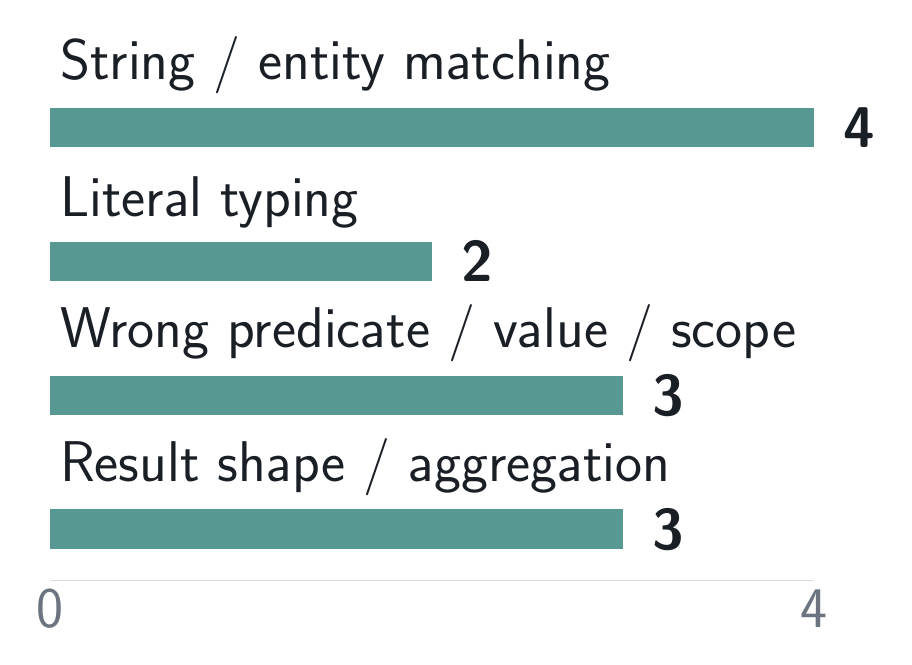
\begin{tikzpicture}[x=0.2\linewidth,y=1mm]
\errbar{51}{4}{String / entity matching}
\errbar{34}{2}{Literal typing}
\errbar{17}{3}{Wrong predicate / value / scope}
\errbar{0}{3}{Result shape / aggregation}
\draw[rulec] (0,-4) -- (4,-4);
\node[anchor=north, font=\SmallF, text=muted] at (0,-4) {0};
\node[anchor=north, font=\SmallF, text=muted] at (4,-4) {4};
\end{tikzpicture}
\end{center}
{\SmallF\textcolor{muted}{All twelve errors, by type; none is a vocabulary or
schema failure.}}

\vspace{-1mm}
\takeaway{Every one of the twelve is visible in the query itself, which is the
property the setting demanded.}}}

\newlength{\rowAht}\newlength{\rowAdp}
\settoheight{\rowAht}{\usebox{\colAbox}}\settodepth{\rowAdp}{\usebox{\colAbox}}
\newlength{\rowBht}\newlength{\rowBdp}
\settoheight{\rowBht}{\usebox{\colBbox}}\settodepth{\rowBdp}{\usebox{\colBbox}}
\newlength{\rowA}\setlength{\rowA}{\dimexpr\rowAht+\rowAdp\relax}
\newlength{\rowB}\setlength{\rowB}{\dimexpr\rowBht+\rowBdp\relax}
\newlength{\rowbase}
\newlength{\padA}
\newlength{\padB}
\ifdim\rowA>\rowB
  \setlength{\rowbase}{\rowA}
\else
  \setlength{\rowbase}{\rowB}
\fi
\setlength{\padA}{\dimexpr\rowbase-\rowA\relax}
\setlength{\padB}{\dimexpr\rowbase-\rowB\relax}

% =====================================================================
%  HEADER
% =====================================================================

\begin{tikzpicture}
  \node[fill=ink, rounded corners=8pt, inner xsep=16mm, inner ysep=14mm,
        text width=\dimexpr\linewidth-32mm\relax, align=left] {%
    \color{white}
    {\TitleF Trust the Query, Not the Answer\par}
    \vspace{4mm}
    {\SubtitleF\color{tealsoft} Auditable Text-to-SPARQL over the GLEIF Register\par}
    \vspace{9mm}
    {\BylineF Jannic Alexander Cutura\quad\textcolor{rulec}{\textbar}\quad
     European Central Bank\quad\textcolor{rulec}{\textbar}\quad DSTI School of Engineering
     \hfill \texttt{github.com/JannicCutura/finnlp-2026}\par}};
\end{tikzpicture}

\vspace{6mm}

% =====================================================================
%  THREE COLUMNS
% =====================================================================
\noindent
% ---------------------------------------------------------------- COL 1
\begin{minipage}[t]{\colw}
\BodyF

\usebox{\colAbox}

\vspace{\padA}
\includegraphics[width=\mapdispw]{../blog/subsidiary_map_poster.pdf}

\vspace{1mm}
\parbox{\mapdispw}{\centering\SmallF\textcolor{muted}{452 direct
subsidiaries of Siemens Aktiengesellschaft, by country of registration --- circle
area proportional to count.}}

\end{minipage}
\hspace{\colgap}
% ---------------------------------------------------------------- COL 2
\begin{minipage}[t]{\colw}
\BodyF

\usebox{\colBbox}

\vspace{\padB}
\vspace{\mapblank}

\end{minipage}
\hspace{\colgap}
% ---------------------------------------------------------------- COL 3
\begin{minipage}[t]{\colw}
\BodyF

\vspace{\wtreserve}
\heading{Benchmark}

144 questions over six tiers, from a specification fixed \emph{before}
instantiation around a KYC analyst, a supervisor and a fund-operations user, in
business language naming no predicate or IRI. Every reference query runs against
the pinned snapshot, so its result cannot drift from the graph. The 54-question
development set drove three schema revisions; the 90-question held-out set came
afterwards, against a frozen prompt.

\vspace{1mm}
\begin{center}{\renewcommand{\arraystretch}{1.15}\TabF
\begin{tabular}{@{}lccc@{}}
\toprule
 & \multicolumn{2}{c}{\textbf{20B}} & \textbf{120B} \\
\cmidrule(lr){2-3}\cmidrule(lr){4-4}
\textbf{Tier} & Dev & Held & Held \\
\midrule
a\ \ lookup           & 10/10 & 10/15 & 12/15 \\
b\ \ single-hop       & 10/10 & 14/14 & 14/14 \\
c\ \ multi-hop        & 8/8   & 13/15 & 14/15 \\
d\ \ attribute filter & 7/7   & 14/15 & 14/15 \\
e\ \ aggregate        & 6/7   & 13/15 & 11/15 \\
f\ \ unanswerable     & 12/12 & 14/16 & 14/16 \\
\midrule
\textbf{Exec.\ accuracy}  & \textbf{98.1\%} & \textbf{86.7\%} & \textbf{87.8\%} \\
\quad 95\% CI             & 90--100 & 78--92 & 79--93 \\
QALD macro-F1             & 0.981 & 0.897 & 0.893 \\
Validity rate             & 100\% & 100\% & 98.9\% \\
First-try / repaired      & 48/6 & 82/8 & 80/9 \\
\bottomrule
\end{tabular}}
\end{center}

\heading{What each part buys}

\vspace{1mm}
\begin{center}
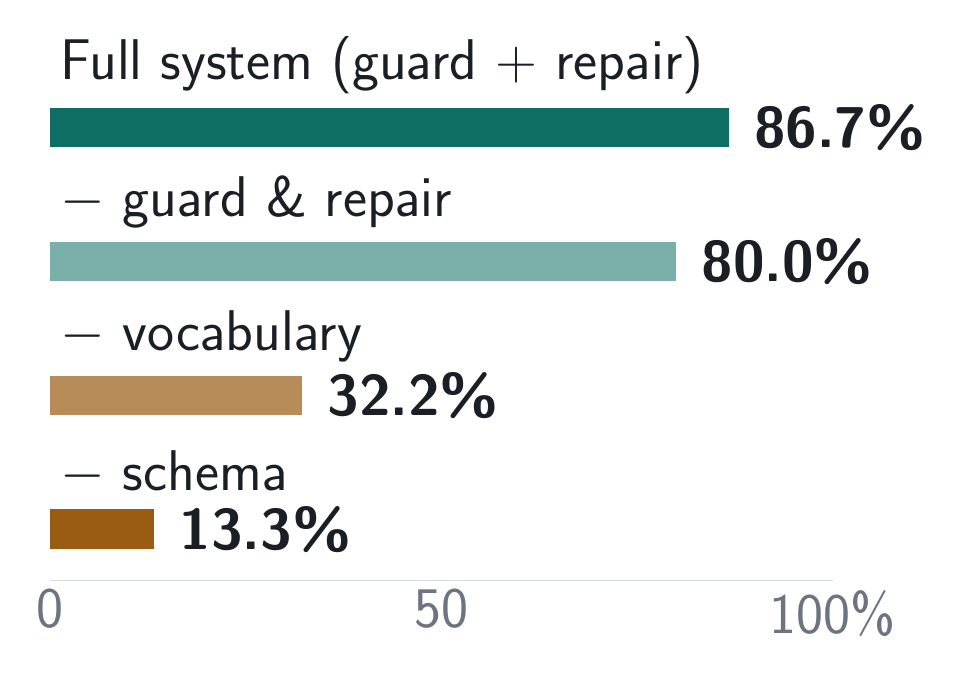
\begin{tikzpicture}[x=0.0082\linewidth,y=1mm]
\abbar{51}{86.7}{Full system (guard + repair)}{teal}
\abbar{34}{80.0}{$-$ guard \& repair}{teal!55}
\abbar{17}{32.2}{$-$ vocabulary}{warm!70}
\abbar{0}{13.3}{$-$ schema}{warm}
\baraxis
\end{tikzpicture}
\end{center}

\vspace{-3mm}
{\SmallF\textcolor{muted}{Held-out accuracy (20B): stripping vocabulary drops it to
32.2\%, stripping schema to 13.3\%. Guard and repair add the last 6.7 points, to
100\% validity.}}

\heading{Models}

\vspace{1mm}
\begin{center}
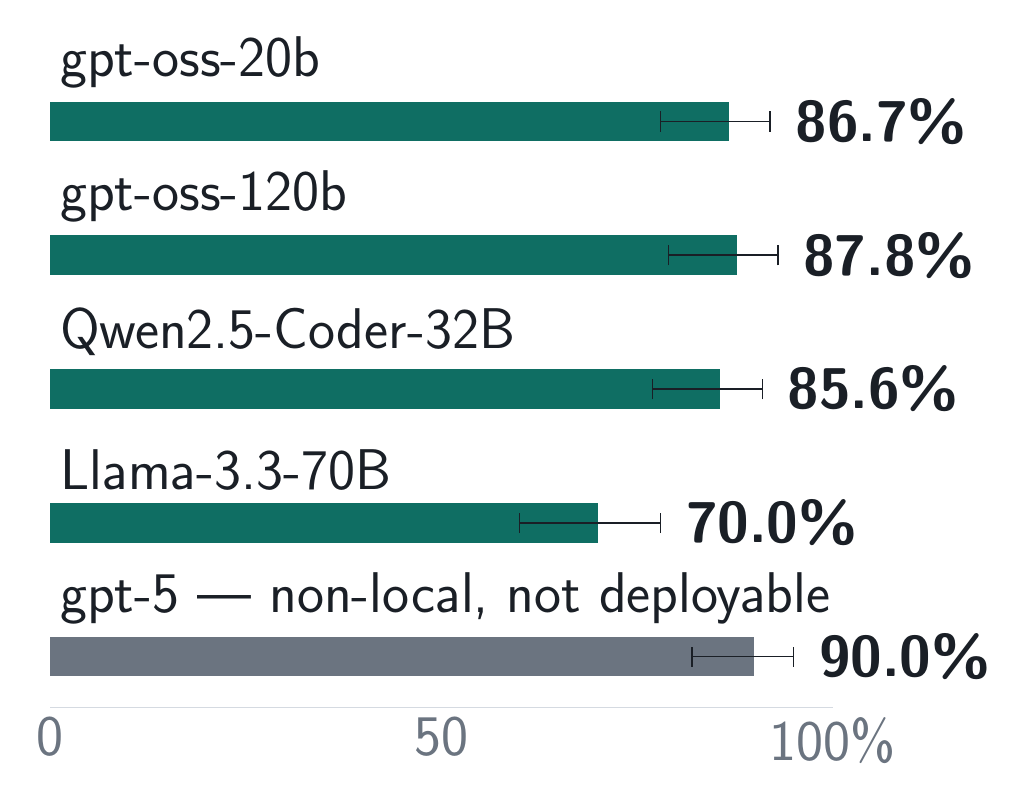
\begin{tikzpicture}[x=0.0082\linewidth,y=1mm]
\modbar{68}{86.7}{78}{92}{gpt-oss-20b}{teal}
\modbar{51}{87.8}{79}{93}{gpt-oss-120b}{teal}
\modbar{34}{85.6}{77}{91}{Qwen2.5-Coder-32B}{teal}
\modbar{17}{70.0}{60}{78}{Llama-3.3-70B}{teal}
\modbar{0}{90.0}{82}{95}{gpt-5 --- non-local, not deployable}{muted}
\baraxis
\end{tikzpicture}
\end{center}

\vspace{-3mm}
{\SmallF\textcolor{muted}{95\% CI whiskers: size is not the bottleneck and open
versus closed is not either; training focus is. The code-tuned models sit inside
one another's intervals, 16 points above the general instruction model.}}

\heading{Limits, and what is next}

144 questions on one graph with a thin schema, one snapshot, one run per model, and
no user study yet. The construction, though, is not specific to corporate
structure: it is a model writing queries against any source described by an
ontology. Real data sits across relational, graph and document stores, each with
its own query language --- extending the same generate--guard--repair loop across
them is the direction we intend to pursue. The nearer-term test is whether the
same guard holds up on a schema an order of magnitude larger, where a single typo
has far more plausible near-misses to repair towards.

\end{minipage}

\vspace{4mm}

% =====================================================================
%  FOOTER
% =====================================================================
\noindent
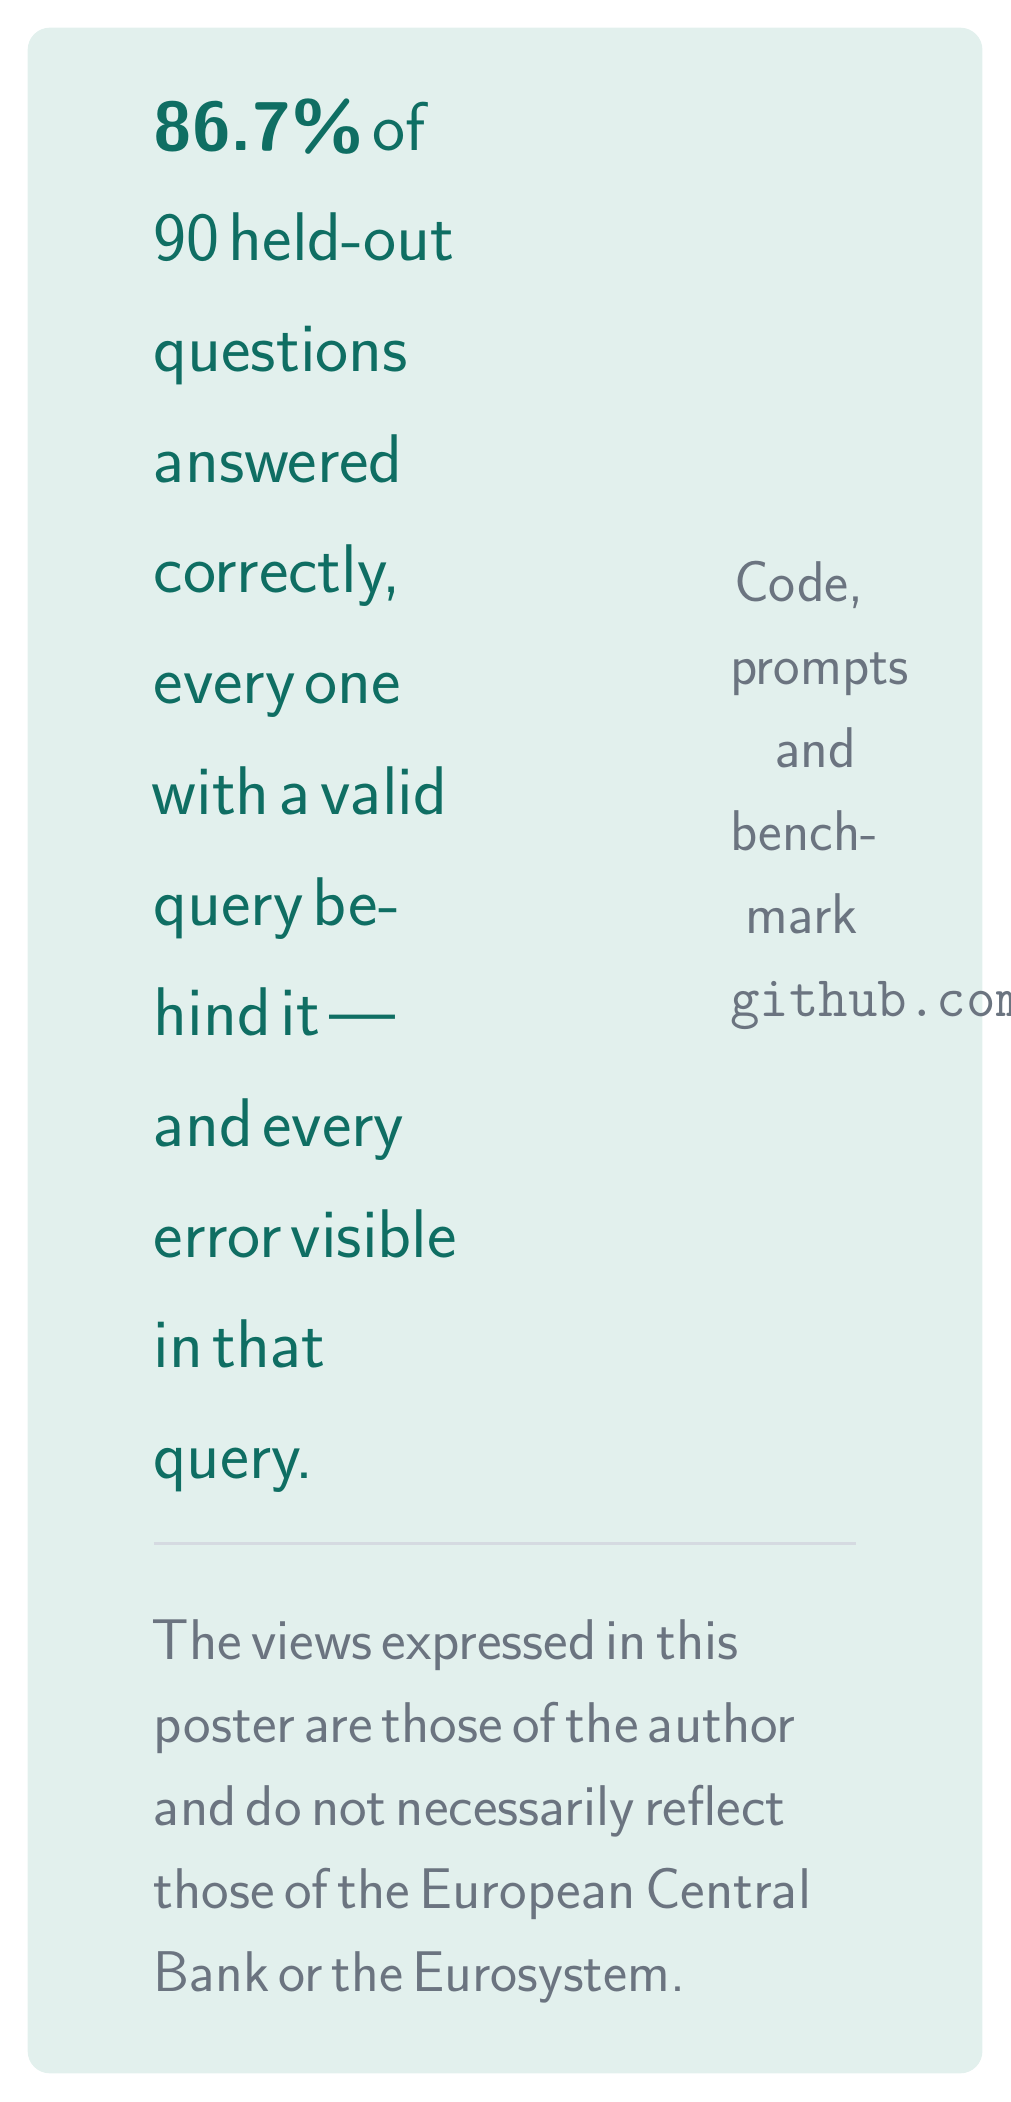
\begin{tikzpicture}
  \node[fill=tealsoft, rounded corners=8pt, inner xsep=16mm, inner ysep=9mm,
        text width=\dimexpr\textwidth-32mm\relax, align=left] {%
    \BylineF
    \begin{minipage}[c]{0.70\dimexpr\textwidth-32mm\relax}
      \textcolor{teal}{\textbf{86.7\%} of 90 held-out questions answered correctly,
      every one with a valid query behind it --- and every error visible in that
      query.}
    \end{minipage}\hfill
    \begin{minipage}[c]{0.28\dimexpr\textwidth-32mm\relax}
      \raggedleft\SmallF\textcolor{muted}{Code, prompts and benchmark\\
      \texttt{github.com/JannicCutura/finnlp-2026}}
    \end{minipage}
    \par\vspace{6mm}
    {\color{rulec}\rule{\linewidth}{1pt}}\par\vspace{4mm}
    {\setlength{\parskip}{0pt}\SmallF\textcolor{muted}{The views expressed in this
     poster are those of the author and do not necessarily reflect those of the
     European Central Bank or the Eurosystem.}\par}};
\end{tikzpicture}

\end{document}
